\documentclass{standalone}
\usepackage{tikz}
\usetikzlibrary{positioning}

\begin{document}
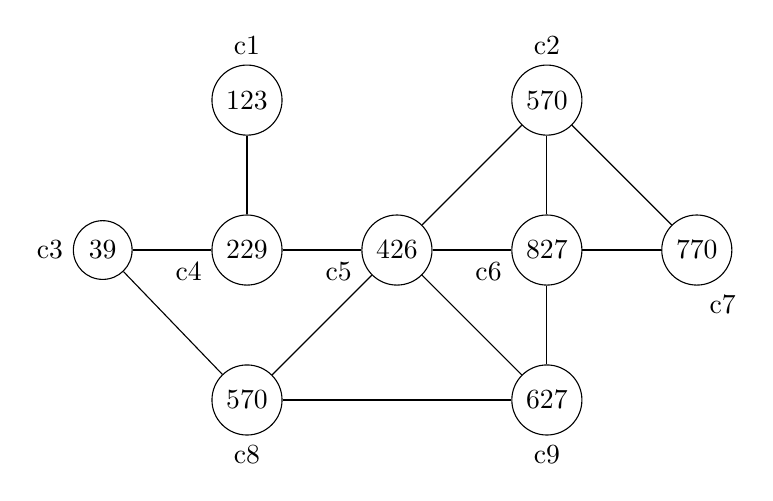
\begin{tikzpicture}
    \node[circle, draw, label=left:c3] (v3) {39}; 
    \node[circle, draw, label=185:c4, right = of v3] (v4) {229}; 
    \node[circle, draw, label=185:c5, right = of v4] (v5) {426}; 
    \node[circle, draw, label=185:c6, right = of v5] (v6) {827}; 
    \node[circle, draw, label=275:c7, right = of v6] (v7) {770}; 
    \node[circle, draw, label=c1, above = of v4] (v1) {123}; 
    \node[circle, draw, label=c2, above = of v6] (v2) {570}; 
    \node[circle, draw, label=below:c8, below = of v4] (v8) {570}; 
    \node[circle, draw, label=below:c9, below = of v6] (v9) {627}; 

    \draw (v1) -- (v4);
    \draw (v2) -- (v6);
    \draw (v6) -- (v9);
    \draw (v3) -- (v4);
    \draw (v4) -- (v5);
    \draw (v5) -- (v6);
    \draw (v6) -- (v7);
    \draw (v3) -- (v8);
    \draw (v8) -- (v5);
    \draw (v5) -- (v2);
    \draw (v2) -- (v7);
    \draw (v5) -- (v9);
    \draw (v8) -- (v9);
\end{tikzpicture}
\end{document}
